\documentclass{beamer}
\usetheme{Dresden}
\usecolortheme{whale}
\usepackage[utf8]{inputenc}
\usepackage[T1]{fontenc}
\usepackage{ragged2e}
\usepackage{amssymb}
\usepackage{booktabs}
\usepackage{graphicx}
\usepackage{mathtools}
\usepackage{commath}
\usepackage{amsmath}
\usepackage{wrapfig}
\usepackage{multicol}
\usepackage{listings}

\newcommand{\nt}{$\underline{\text{Note}}:$ }
\newcommand{\ex}{$\underline{\text{Example}}:$ }
\newcommand{\rem}{$\underline{\text{Recall}}:$ }
\newcommand{\rmk}{$\underline{\text{Remark}}:$ }
\newcommand{\tab}{\quad}
\newcommand{\nll}{\\\vspace{2ex}}

\graphicspath{ {images/} }

\lstset{
    basicstyle=\ttfamily\scriptsize,
    keywordstyle=\color{blue!70!black},
    commentstyle=\color{gray},
    breaklines=true,
    frame=single,
    backgroundcolor=\color{gray!5},
}

\title[Voice Scribe v3]{Voice Scribe v3\\Desktop Application}
\author[J. Yanez]{Johnraymond Yanez}
\institute[Voice Scribe]{Voice Scribe}
\date{\today}

\begin{document}


% -- Title -----------------------------------------------------------------
\begin{frame}
\small{\titlepage}
\end{frame}


% -- Overview --------------------------------------------------------------
\begin{frame}{Overview}
    \begin{itemize}
        \item \textbf{Context} --- v1 and v2 in brief
        \item \textbf{The Platform Ceiling} --- what the browser cannot close
        \item \textbf{v3 Architecture} --- Tauri, Python sidecar, platform layer
        \item \textbf{Roadmap} --- five sub-milestones (v3.0--v3.4)
        \item \textbf{Key Design Decisions} --- the choices and why
        \item \textbf{Prerequisites \& Deferrals}
    \end{itemize}
\end{frame}


% =========================================================================
\section{Context}
% =========================================================================

\begin{frame}{v1 --- The Primitive (2026-04-02)}
    \small
    \textbf{Goal:} local speech-to-text that never leaves the machine.

    \vspace{0.4em}
    \textbf{What shipped:}
    \begin{itemize}\setlength{\itemsep}{2pt}
        \item Record one utterance in the browser; POST to a local container
        \item ffmpeg transcodes; faster-whisper (large-v3, GPU) infers
        \item Transcript returned to an editable textarea; one-click copy
        \item CPU fallback (\texttt{small} model) validated
    \end{itemize}

    \vspace{0.3em}
    \textbf{What it proved:} a two-service localhost architecture --- React on the host,
    FastAPI in Docker --- can deliver accurate, private transcription with no cloud dependency
    and no round-trip latency beyond the GPU itself.

    \vspace{0.3em}
    \textbf{Intentionally out of scope:} streaming, continuous recording, hotkeys, voice
    commands, server-side persistence. v1 was a primitive, not a product.
\end{frame}


\begin{frame}{v2 --- The Interaction Model (2026-04-04)}
    \small
    Built on v1 across four sequenced milestones:

    \vspace{0.3em}
    \begin{table}
    \centering\footnotesize
    \begin{tabular}{@{} l p{7.8cm} @{}}
        \toprule
        \textbf{Milestone} & \textbf{Key deliverable} \\
        \midrule
        v2.0 & Hotkey system (\texttt{Ctrl+Shift+*}); settings panel with
               live model swap (threading-safe, VRAM cleanup) \\
        v2.1 & WebSocket streaming default; words appear as segments complete;
               HTTP POST fallback automatic \\
        v2.2 & Continuous recording; client-side VAD (Silero v4/WASM);
               paragraph breaks; drain-then-done \\
        v2.3.x & Voice commands: \texttt{copy} and \texttt{clear} as single-word
                 exact-segment matches; paragraph break timing fixed \\
        \bottomrule
    \end{tabular}
    \end{table}

    \vspace{0.3em}
    \textbf{What it proved:} streaming, browser-side ML inference, and voice-driven control
    all work reliably at the browser layer. The interaction model is validated.

    \vspace{0.1em}
    \textbf{What it could not close:} covered next.
\end{frame}


% =========================================================================
\section{The Platform Ceiling}
% =========================================================================

\begin{frame}{What the Browser Cannot Do}
    \small
    v2 delivers a capable continuous dictation tool. One constraint cannot be engineered around:

    \vspace{0.4em}
    \begin{block}{The Clipboard Focus Rule}
        \texttt{navigator.clipboard.writeText()} requires the browser tab to have
        document focus. If the user has switched to another application ---
        which is the entire point of a transcription tool --- the write is blocked.
    \end{block}

    \vspace{0.4em}
    This is a security boundary enforced by the browser platform. Not a missing feature.
    Workarounds are fragile and non-portable.

    \vspace{0.3em}
    VAD and recording work cross-window --- Voice Scribe listens while the user works
    elsewhere. \textbf{Delivery is what breaks.} The full loop requires native OS access.
\end{frame}


\begin{frame}{The Delivery Gap --- Diagram}
    \begin{center}
    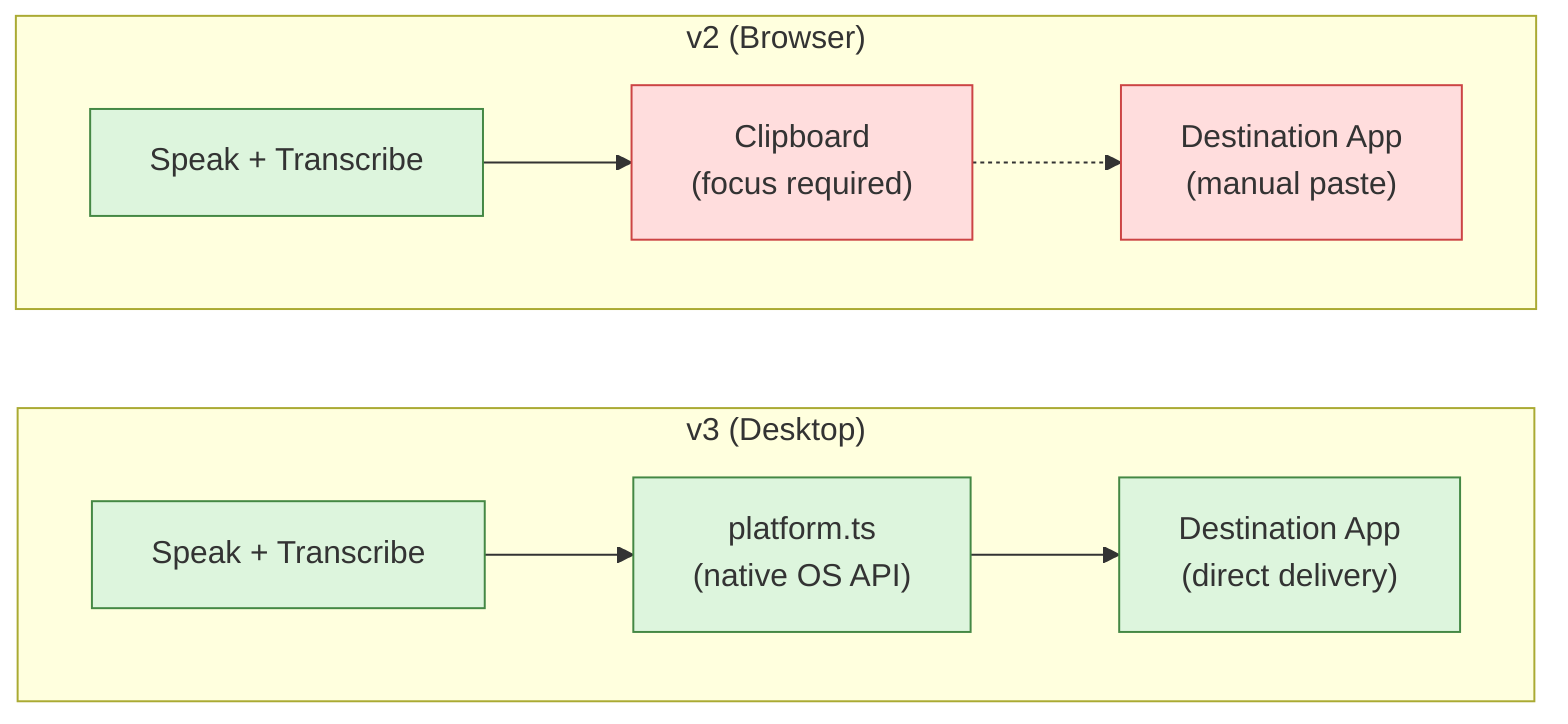
\includegraphics[width=0.95\textwidth,keepaspectratio]{images/delivery-gap.png}
    \end{center}

    \vspace{0.3em}
    {\scriptsize
    \textcolor{green!50!black}{Green} = works as intended. \quad
    \textcolor{red!60!black}{Red} = browser platform ceiling. \quad
    v3 closes the last step.}
\end{frame}


% =========================================================================
\section{v3 Architecture}
% =========================================================================

\begin{frame}{System Architecture at v3}
    \small
    v3 is a platform change, not a rewrite. The same React frontend and Python backend
    are wrapped in a Tauri desktop application.

    \vspace{0.3em}
    \begin{itemize}\setlength{\itemsep}{3pt}
        \item \textbf{Tauri} hosts the Vite/React frontend in a native webview ---
              the same build, no component forks
        \item \textbf{Python sidecar} replaces Docker --- Tauri spawns
              \texttt{uvicorn app.main:app} as a managed child process
        \item \textbf{\texttt{platform.ts}} routes platform-conditional behavior
              at the service layer --- clipboard, injection, context detection
        \item \textbf{No Docker dependency} at runtime --- the model runs bare
              on the host GPU; Docker path (\texttt{make dev}) remains for web
              development
    \end{itemize}

    \vspace{0.2em}
    \begin{block}{What is unchanged}
        \small All of v2: push-to-talk, continuous mode, VAD, streaming, voice commands
        (\texttt{copy}, \texttt{clear}), settings panel, hotkeys. The browser
        build continues to work without modification.
    \end{block}
\end{frame}


\begin{frame}{Architecture --- Diagram}
    \begin{center}
    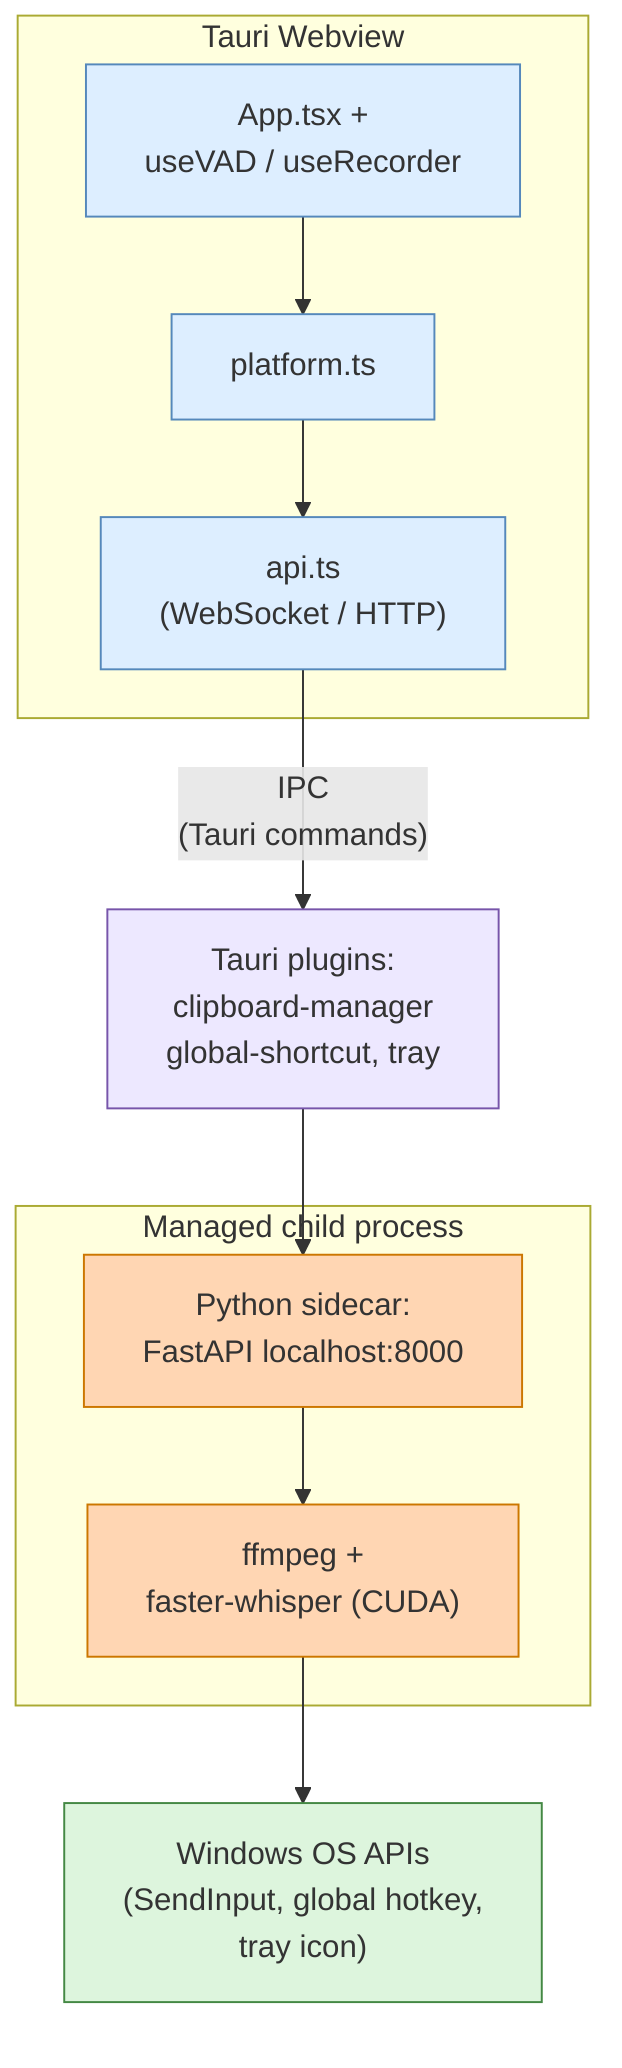
\includegraphics[height=0.72\textheight,keepaspectratio]{images/v3-architecture.png}
    \end{center}

    {\scriptsize
    \textcolor{blue!50!black}{Blue} = React webview \quad
    \textcolor{orange!70!black}{Orange} = Python sidecar \quad
    \textcolor{violet!60!black}{Lavender} = Tauri plugins \quad
    \textcolor{green!50!black}{Green} = OS APIs.}
\end{frame}


\begin{frame}{Monorepo Structure}
    \small
    One repository, three app directories. The API is shared between web and desktop.

    \vspace{0.3em}
    \begin{columns}[T]
        \begin{column}{0.52\textwidth}
            \footnotesize
            \textbf{\texttt{apps/web/}} --- unchanged. Vite frontend.
            Serves both browser tabs and the Tauri webview.

            \vspace{0.35em}
            \textbf{\texttt{apps/api/}} --- unchanged. FastAPI backend.
            v2: runs in Docker. v3: runs as a managed
            sidecar. Same code, different launch context.

            \vspace{0.35em}
            \textbf{\texttt{apps/desktop/}} --- new. Contains
            \texttt{tauri.conf.json} and \texttt{src-tauri/}
            (Rust config and Tauri commands) \emph{only}.
            No component copies live here.
        \end{column}
        \begin{column}{0.44\textwidth}
            \begin{block}{The Fork Rule}
                \footnotesize
                Two copies of a component are two maintenance
                surfaces that diverge silently.

                Capability differences (native clipboard,
                direct injection) live in
                \texttt{platform.ts} --- not in component
                forks and not in a parallel service file.

                If you find yourself copying a component
                into \texttt{apps/desktop/}, stop.
            \end{block}
        \end{column}
    \end{columns}
\end{frame}


\begin{frame}{\texttt{platform.ts} --- The Service Layer}
    \small
    The single routing surface for all platform-conditional behavior.
    Components call \texttt{platform.*} and are unaware of context.

    \vspace{0.3em}
    \begin{table}
    \centering\scriptsize
    \begin{tabular}{@{} l p{3.6cm} p{3.6cm} @{}}
        \toprule
        \textbf{Export} & \textbf{Browser} & \textbf{Tauri (Desktop)} \\
        \midrule
        \texttt{isDesktop()} &
            Returns \texttt{false} &
            Returns \texttt{true}
            (\texttt{window.\_\_TAURI\_\_}) \\[4pt]
        \texttt{writeClipboard()} &
            \texttt{navigator.clipboard} \texttt{.writeText()} &
            \texttt{fetch()} POST to \texttt{:8001} ---
            Rust writes via \texttt{arboard} \\[4pt]
        \texttt{submitText()} &
            Calls \texttt{writeClipboard()} &
            Calls \texttt{writeClipboard()} (direct injection deferred) \\[4pt]
        \texttt{emitRecordingState()} &
            No-op &
            Emits \texttt{recording-state-changed} to Rust (tray tooltip sync) \\
        \bottomrule
    \end{tabular}
    \end{table}

    \vspace{0.2em}
    {\footnotesize\textbf{Build contract:} One Vite build, one artifact. Desktop clipboard
    uses \texttt{fetch()} to a Rust HTTP server --- no Tauri plugin imports needed.
    Browser build produces zero import errors.}
\end{frame}


% =========================================================================
\section{Roadmap}
% =========================================================================

\begin{frame}{Milestone Timeline}
    \begin{center}
    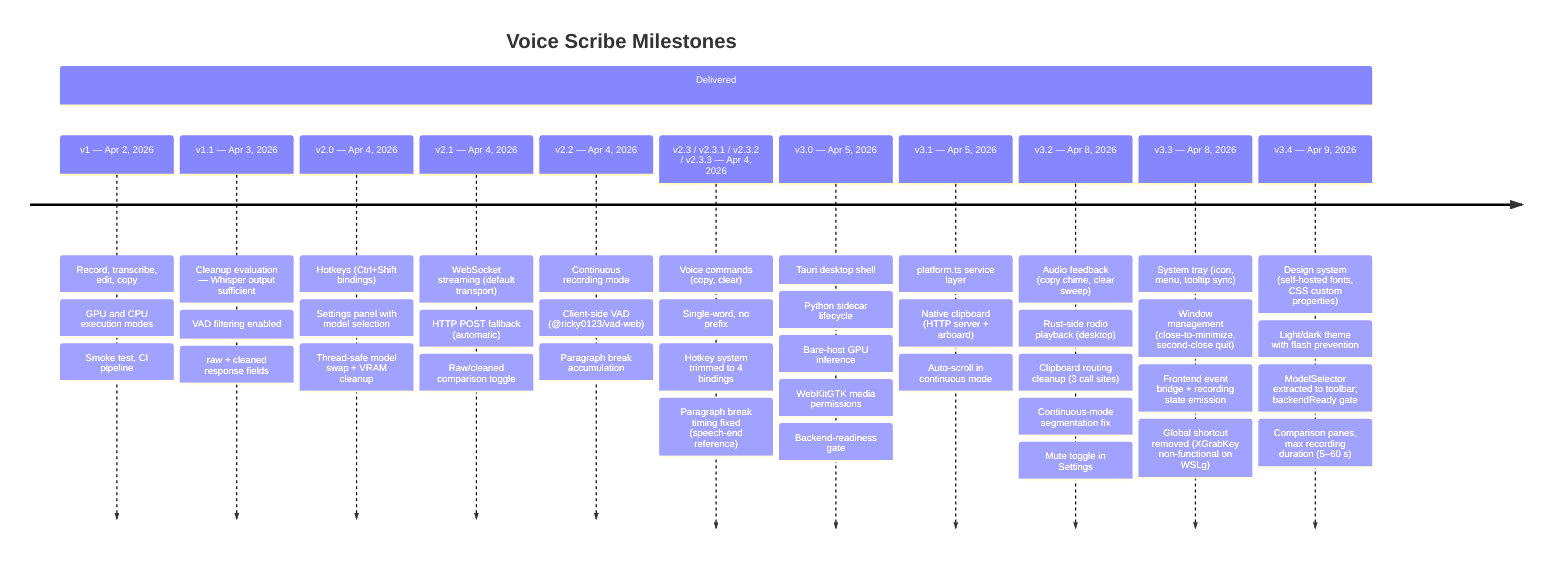
\includegraphics[width=0.95\textwidth]{images/milestone-timeline.png}
    \end{center}

    {\scriptsize Delivered milestones show actual dates and key outputs.
    Planned milestones show sequence --- no hard deadlines.}
\end{frame}


\begin{frame}{v3.0 --- Tauri Shell + Sidecar Lifecycle}
    \small
    \textbf{Deliverable:} Tauri app launches, manages the Python sidecar, all v2
    functionality works identically to the browser version.

    \vspace{0.2em}
    \textbf{Key scope:}
    \begin{itemize}\setlength{\itemsep}{0pt}
        \item \texttt{apps/desktop/} scaffolding: Tauri v2 CLI, \texttt{tauri.conf.json},
              Cargo project
        \item Sidecar lifecycle: startup health poll, graceful shutdown (SIGTERM $\to$
              SIGKILL after timeout), crash surface, port-conflict error dialog
        \item \texttt{config.py} defaults for host: \texttt{\textasciitilde/.cache/voice-scribe},
              system temp dir, Tauri webview CORS origin
        \item WebSocket origin enforcement updated; \texttt{make desktop} target added
    \end{itemize}

    \vspace{0.2em}
    \textbf{Gate:} record $\to$ transcribe $\to$ display via WebSocket (primary) and
    HTTP POST (fallback). Close app $\to$ no orphan \texttt{uvicorn} process.
    Relaunch works clean.

    \textbf{Not in scope:} native clipboard, \texttt{submit}, global hotkeys, system tray.
\end{frame}


\begin{frame}{v3.1 --- Native Clipboard + Auto-Scroll}
    \small
    \textbf{Deliverable:} \texttt{copy} voice command and \texttt{Ctrl+Shift+Y} use native
    OS clipboard. No window focus required.

    \vspace{0.15em}
    \textbf{Key scope:}
    \begin{itemize}\setlength{\itemsep}{0pt}
        \item \texttt{platform.ts} introduced: \texttt{isDesktop()},
              \texttt{writeClipboard()}, \texttt{submitText()} stub
        \item Two \texttt{App.tsx} clipboard call sites routed through
              \texttt{platform.writeClipboard()}
        \item HTTP clipboard server (\texttt{tiny\_http} + \texttt{arboard}
              on port 8001) --- bypasses WebKitGTK user-activation requirement
        \item \texttt{voiceCommands.ts} unchanged; \texttt{submit} deferred
        \item Auto-scroll in continuous mode: pins to bottom on new segments
    \end{itemize}

    \vspace{0.1em}
    \textbf{Gate:} dictate $\to$ say ``copy'' $\to$ switch to VS Code $\to$ Ctrl+V $\to$
    transcript is there. Same with Ctrl+Shift+Y. Browser build: zero import errors,
    all tests pass.
\end{frame}


\begin{frame}{v3.2 --- Audio Feedback + Clipboard + Segmentation (2026-04-08)}
    \small
    \textbf{Deliverable:} audible voice command confirmation. Clipboard consolidation.
    Clean continuous-mode segment joins.

    \vspace{0.2em}
    \textbf{What shipped:}
    \begin{itemize}\setlength{\itemsep}{0pt}
        \item \texttt{copy}: ascending chime after \texttt{writeClipboard()} succeeds;
              silence on failure. \texttt{clear}: descending sweep on state clear
        \item Browser: \texttt{HTMLAudioElement}. Desktop: \texttt{rodio} via Rust
              HTTP server on port 8001 (same WebKitGTK bypass as clipboard)
        \item Mute toggle in Settings; all three clipboard call sites through
              \texttt{platform.writeClipboard()}
        \item Segment joins: space on short pause, paragraph break on long pause
    \end{itemize}

    \vspace{0.1em}
    {\footnotesize\textbf{Pattern:} \texttt{rodio} added after WebKitGTK audio proved
    unreliable. Two OS-level operations (clipboard, audio) now bypass the webview
    via the Rust HTTP server --- an established architectural pattern, not two
    individual workarounds.}
\end{frame}


\begin{frame}{v3.3 --- System Tray + Window Management (2026-04-08)}
    \small
    \textbf{Deliverable:} Voice Scribe runs in the background. System tray provides
    status and quick access. Window close minimizes; sidecar stays alive.

    \vspace{0.2em}
    \textbf{What shipped:}
    \begin{itemize}\setlength{\itemsep}{0pt}
        \item System tray: icon, context menu (Toggle Recording, Settings, Quit),
              recording-state tooltip, left-click window toggle
        \item Close-to-minimize with second-close quit; three sidecar cleanup paths
        \item Frontend event bridge: tray events route through the same
              \texttt{handleToggleRecording} as the UI button
        \item \texttt{emitRecordingState()} in \texttt{platform.ts} syncs tray
              tooltip on every state transition
    \end{itemize}

    {\footnotesize\textbf{Scope reduction:} Global shortcut plugin implemented and removed ---
    \texttt{XGrabKey} does not deliver events on WSLg. Event bridge retained;
    re-adding the plugin on native Linux is a Rust-only change.
    \texttt{Ctrl+Shift+Y}/\texttt{X} work in the desktop webview via \texttt{useHotkeys}.}
\end{frame}


\begin{frame}{v3.4 --- Design System + UI Refresh (2026-04-09)}
    \small
    \textbf{Deliverable:} Coherent visual identity, persistent light/dark theme,
    and model selection in the primary toolbar.

    \vspace{0.15em}
    \textbf{What shipped:}
    \begin{itemize}\setlength{\itemsep}{0pt}\footnotesize
        \item \textbf{Design system} --- self-hosted fonts (Hanken Grotesk, Crimson Pro);
              CSS custom properties for all color tokens; warm utilitarian palette
        \item \textbf{Light/dark theme} --- flash-prevention script in
              \texttt{index.html}; toolbar toggle; persisted to \texttt{localStorage}
        \item \textbf{\texttt{ModelSelector.tsx}} extracted from Settings into the
              toolbar; gates fetch on \texttt{backendReady}; swap status inline
        \item \textbf{Layout + comparison} --- three-zone layout; Recorder compacted
              into toolbar; Raw/Edit comparison panes with per-pane copy buttons
        \item \textbf{Settings + duration} --- accessible during recording; max
              recording duration (push-to-talk, 5--60\,s; capped to backend limit)
    \end{itemize}

    \vspace{0.1em}
    {\footnotesize\textbf{178 tests} (134 frontend + 44 backend).
    No backend changes. v3.4 is the last mainline milestone.}
\end{frame}


% =========================================================================
\section{Key Design Decisions}
% =========================================================================

\begin{frame}{Why Python Sidecar, Not Rust Inference?}
    \small
    \begin{columns}[T]
        \begin{column}{0.54\textwidth}
            \textbf{The decision}

            Tauri spawns the existing FastAPI backend as a managed child process.
            No Docker. No rewrite of the inference layer.

            \vspace{0.4em}
            \textbf{Why not rewrite in Rust?}
            \begin{itemize}\setlength{\itemsep}{1pt}
                \item faster-whisper is proven --- accuracy and
                      speed validated in production use
                \item Building the Tauri shell \textit{and}
                      rewriting inference simultaneously is
                      scope explosion
                \item The two problems are independent and
                      can be sequenced
            \end{itemize}
        \end{column}
        \begin{column}{0.42\textwidth}
            \begin{block}{When to revisit}
                \footnotesize
                Rust-native inference (whisper.cpp) is a
                \textbf{named future milestone}.

                Trigger: distribution to non-developer
                users becomes a requirement.

                Single-binary packaging is the forcing
                function --- not performance.

                Until then, the Python sidecar is
                the correct decision, not technical debt.
            \end{block}
        \end{column}
    \end{columns}
\end{frame}


\begin{frame}{Why Runtime Detection, Not Build Flags?}
    \small
    \textbf{The decision:} one Vite build serves both the browser and the Tauri webview.
    Platform context detected at runtime, not build time.

    \vspace{0.4em}
    \begin{itemize}\setlength{\itemsep}{3pt}
        \item \textbf{\texttt{window.\_\_TAURI\_\_}} --- injected by Tauri into the webview.
              Absent in the browser. \texttt{platform.ts} reads this at call time, not
              at bundle time.

        \item \textbf{No Tauri imports in the clipboard or audio path} --- desktop
              clipboard and audio use \texttt{fetch()} to a Rust HTTP server, not
              Tauri plugins. No \texttt{@tauri-apps/} imports in the production build.

        \item \textbf{Event bridge uses \texttt{window.\_\_TAURI\_\_}} --- tray menu
              actions and recording state sync use the global Tauri object
              (\texttt{emit}/\texttt{listen}), not plugin crates. Available at
              runtime in the webview, absent in the browser --- same detection
              pattern as \texttt{isDesktop()}.
    \end{itemize}

    \vspace{0.3em}
    \textbf{What this avoids:} separate build targets, separate environment variables,
    build-time divergence. One artifact to test, one to ship.
\end{frame}


\begin{frame}{Why \texttt{copy} and \texttt{submit} Are Separate Commands}
    \small
    \begin{table}
    \centering\footnotesize
    \begin{tabular}{@{} l p{3.9cm} p{3.9cm} @{}}
        \toprule
        & \textbf{\texttt{copy}} & \textbf{\texttt{submit}} \\
        \midrule
        Action    & Writes to clipboard      & Injects keystrokes into focused app \\
        Reversible & Yes                     & No --- undo may be limited \\
        Focus req. & None (native API)       & Previous window must be correct \\
        Risk       & Overwrites clipboard    & May type into wrong application \\
        Browser    & \texttt{navigator.clipboard} & Falls back to \texttt{copy} \\
        \bottomrule
    \end{tabular}
    \end{table}

    \vspace{0.3em}
    Collapsing \texttt{copy} and \texttt{submit} into one command removes the user's
    safe fallback. \texttt{copy} is predictable. \texttt{submit} is irreversible.

    \vspace{0.2em}
    The \textbf{command separation is non-negotiable}.
    The \textbf{specific words} are subject to gate evaluation before each milestone ships.
\end{frame}


% =========================================================================
\section{Prerequisites \& Deferrals}
% =========================================================================

\begin{frame}{Prerequisites Before v3.0}
    \small
    \textbf{Prereq 1 --- \texttt{wsCleanupRef} refactor.}
    Standalone PR on \texttt{main} before any Tauri code exists.

    \begin{itemize}\setlength{\itemsep}{0pt}
        \item Current: single ref, only the last WebSocket cleanup survives.
              Low-risk in-browser (SPA never navigates).
        \item v3 risk: Tauri webview persists; ``close the panel'' is a real unmount.
              Orphaned connections become real.
        \item Fix: \texttt{Set<() => void>} --- register on open, deregister on close,
              iterate on unmount. Browser-tested before \texttt{apps/desktop/} exists.
    \end{itemize}

    \vspace{0.2em}
    \textbf{Prereq 2 --- Host environment validation.}
    The API currently runs in Docker. v3 runs it bare on the host.

    \begin{itemize}\setlength{\itemsep}{0pt}
        \item Python 3.10+, faster-whisper, ffmpeg on \texttt{PATH}, CUDA toolkit
        \item API starts without Docker; \texttt{GET /health} returns
              \texttt{"device": "gpu"}
        \item Close condition: setup documented in \texttt{docs/v3-host-setup.md}
    \end{itemize}
\end{frame}


\begin{frame}{What Is Deferred (Named, Not Forgotten)}
    \small
    \begin{itemize}\setlength{\itemsep}{2pt}
        \item \textbf{Model management UI} --- download progress, cache management.
              Toolbar model selector handles runtime swap; sufficient for v3.0--v3.4.

        \item \textbf{\texttt{submit} (direct injection)} --- deferred indefinitely.
              Downstream products use command draft/staging, not keystroke injection.
              \texttt{submitText()} stub remains as an architectural placeholder.

        \item \textbf{Global shortcut (OS-level hotkey)} --- implemented and removed
              in v3.3. \texttt{XGrabKey} does not deliver events on WSLg's XWayland.
              Event bridge wired and tested; re-addition is a Rust-only change when
              validated on native Linux.

        \item \textbf{Auto-update} --- Tauri built-in. Not in scope for v3.

        \item \textbf{Rust-native inference} --- single-binary distribution trigger.
    \end{itemize}
\end{frame}


\end{document}
